При разработке программы для программно-аппаратной системы Arduino была использована IDE Arduino 1.6.4 как наиболее простой вариант для компиляции и прошивки программы в память микроконтроллера. IDE Arduino представляет собой свободное программное обеспечение для разработки управляющих программ платформы Arduino.

При разработке программного модуля общения ToF-устройства с ЭВМ, была использована Microsoft Visual Studio 2013 Community --- свободная среда разработки от корпорации Microsoft с возможностью разработки на многих языках, включая Arduino, а также под многие платформы, включая .NET и Android.

Функциональная схема обоих программных модулей представлена на рисунке~\ref{fig:softwarefunc}.

\begin{figure}[ht]
    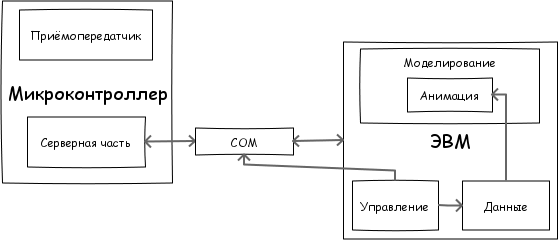
\includegraphics[width=.8\linewidth]{Figures/softwarefunc.png}
    \caption{Функциональная схема программных модулей}
    \label{fig:softwarefunc}
\end{figure}
